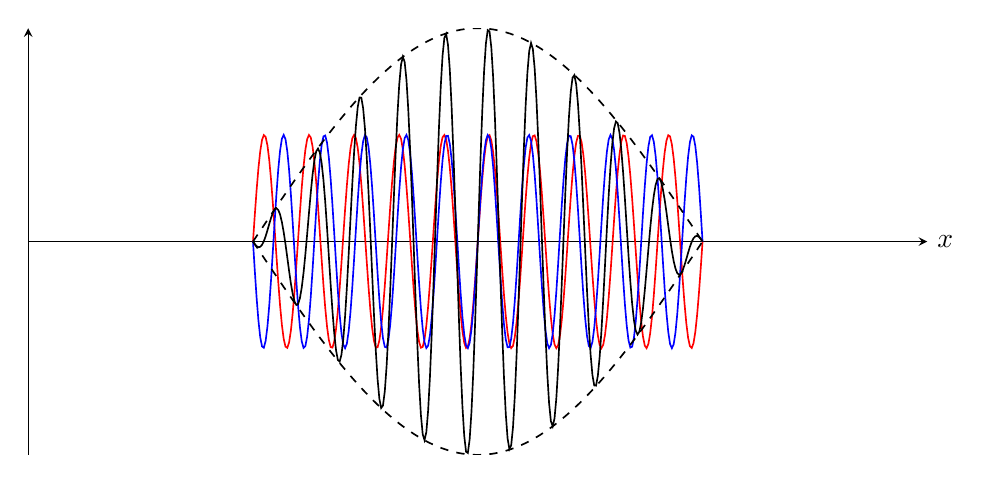
\begin{tikzpicture}
\begin{axis}[
    width=13cm, 
    height=7cm,
    axis x line=center, 
    axis y line=middle, 
    xlabel={$x$},
     x label style={at={(current axis.right of origin)}, right},
    samples=250,
    ymin=-2, ymax=2,
    xmin=0, xmax=20,
    domain=5:15,
    ticks=none
]
\addplot [mark=none, semithick, red] {sin(deg(2*pi*x))};
\addplot [mark=none, semithick, blue] {sin(deg(2*pi*x*1.1))};
\addplot [mark=none, semithick, black] {sin(deg(2*pi*x))+sin(deg(2*pi*x*1.1))};
\addplot [mark=none, semithick, dashed] { 2*cos(deg(2*pi*x*0.05))};
\addplot [mark=none, semithick, dashed] {-2*cos(deg(2*pi*x*0.05))};
\end{axis}
\end{tikzpicture}
